\subsubsection{Asset}\label{sssc:asset}
The \textit{Asset} class is essential to the system, as it represents the real world assets that are to be managed. The class contains the asset's name, a description, an identifier to help identify the physical asset e.g. by using a barcode scanner, and the id of the department it belongs to. The asset also inherits from the \textit{FieldContainer} class, which contains a list of fields on the object. The class also contains an id as well as the date of creation and last update, which is inherited from the \textit{Model} class. The asset does not contain a list of tags, as the relation between asset and tag is a many to many relation and is thus stored separately in the database. 
\par
Aside form these properties the model also contains a few methods for creating a hash code for the asset, compare the asset to another object, and deserializing the assets fields from a JSON format, respectively. 

\todo[inline]{Lav diagram over Asset klassen}

\subsubsection{Tag}\label{sssc:tag}
The \textit{Tag} is one of the core components of the program, as it allows the user to describe assets as well as their states and relations. In the system these are defined in the interface \textit{ITagable}, which \textit{Tag} implements. This interface is implemented by the \textit{User} class (see \autoref{sssc:Users}) as well, as both tag and user can be attached to assets. 
\par

The \textit{Tag} class contains a \textit{Name}, \textit{Fields} and potentially a relation to a parent-tag by way of the id of the parent tag. Parent tags are used to group tags, to make them easier to navigate and use. The relation between a parent and a child tag is a many to one relation stored in the database.
\par
As seen on \autoref{fig:TagClass} the \textit{Tag} class contains the \textbf{Id}, \textbf{CreatedAt} and \textbf{UpdatedAt}, which are inherited from the \textit{Model} class. Besides this the \textit{Tag} class also contains a \textbf{FieldList}, a \textbf{Color} property and the Id of its parent. 
\par \todo{It also contains a department}
The relation between an \textit{Asset} and a \textit{Tag} is defined in a relational database, containing the ID's of the connected tags and assets.

\begin{figure}[H]
    \centering
    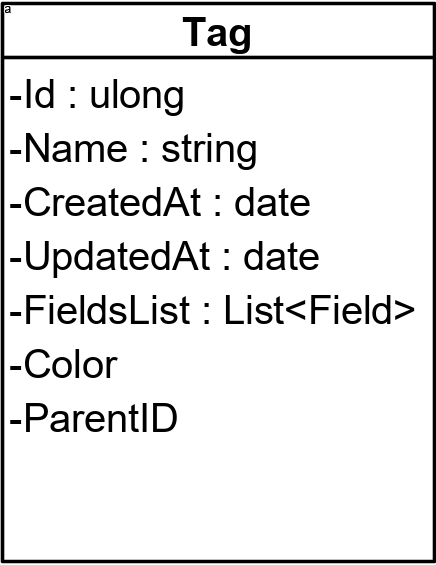
\includegraphics[width=0.2\textwidth]{figures/Implementation/Models/Tag.PNG}
    \caption{Tag class}
    \label{fig:TagClass}
\end{figure}



\subsubsection{User} \label{sssc:Users}
Like the \textit{Tag} class, the \textit{User} class implements the interface \textit{ITagable} and mostly functions as a \textit{Tag}. The relation created when tagging a user onto an asset takes the place of the loan class mentioned in \autoref{ch:problemdomain}, hereby any generalized description of assets can be done via tags. 